% David Shiga and Victor Zabalza
% package vs sub-package

\documentclass[traditabstract]{aa}

\usepackage{graphicx}
\usepackage{xspace}
\usepackage{natbib}
\usepackage{url}
\usepackage[xindy, toc, hyperfirst=false, nolist, nostyles, sanitize={name=false,description=false,symbol=false}]{glossaries}
\bibpunct{(}{)}{;}{a}{}{,}

\newcommand{\astropy}{\texttt{astropy}\xspace}

\begin{document}

% Reading the glossary
% Glossary for the Astropy papers
\newglossaryentry{astropy}{name=astropy, text=astropy}
\newglossaryentry{numpy}{name=NumPy, text=NumPy, description=Numerical Python, first=NumPy \citep{oliphant2006guide,van2011numpy}}
\newglossaryentry{scipy}{name=SciPy, text=SciPy, description={Scientific Python \cite{Jones:2001fk}}, first=SciPy \citep{jones2001scipy}}
\newglossaryentry{matplotlib}{name=Matplolib, text=Matplotlib}
\newglossaryentry{ipython}{name=IPython, text=IPython}
\newglossaryentry{python}{name=python, text=Python, description={Python programming language}}
\newglossaryentry{pandas}{name=pandas, text=pandas}
\newglossaryentry{wcs}{name=wcs, text=WCS, first=World Coordinate System WCS}

\titlerunning{Astropy}
\authorrunning{The Astropy Collaboration}

\title{Astropy: A Community Python Package for Astronomy}

% The author list is not final, and the order of authors may still change.
% Additional authors may be added based on non-commit-based contributions to
% the project.

% Please wrap text to 78 characters.

% I have indicated authors who have acknowledged authorsip by '%confirmed' next
% to their name.

\author{
The Astropy Collaboration
  \and
% Coordination committee
Erik J. Tollerud\inst{\ref{inst:yale}}  % confirmed
  \and
Thomas P. Robitaille\inst{\ref{inst:mpia}}  % confirmed
  \and
Perry Greenfield\inst{\ref{inst:stsci}}  % confirmed
  \and
% Developers (other than coordination committee).
Michael Droettboom\inst{\ref{inst:stsci}}  % confirmed
  \and
Tom Aldcroft\inst{\ref{inst:cfa}}  % confirmed
  \and
Erik Bray\inst{\ref{inst:stsci}}
  \and
Matt Davis\inst{\ref{inst:stsci}}  % confirmed
  \and
Adam Ginsburg\inst{\ref{inst:colorado}}  % confirmed
  \and
Adrian M. Price-Whelan\inst{\ref{inst:columbia}}  % confirmed
  \and
Wolfgang Kerzendorf\inst{\ref{inst:toronto}}
  \and
Alexander Conley\inst{\ref{inst:colorado}}
  \and
Neil Crighton\inst{\ref{inst:mpia}}  % confirmed
  \and
Kyle Barbary\inst{\ref{inst:argonne}}  % confirmed
  \and
Demitri Muna\inst{\ref{inst:osu}}  % confirmed
  \and
Henry Ferguson\inst{\ref{inst:stsci}}
  \and
Frederic Grollier
  \and
Prasanth H. Nair\inst{\ref{inst:freelance}}  % confirmed
  \and
Hans M. G\"unther\inst{\ref{inst:cfa}}  % confirmed
  \and
Christoph Deil\inst{\ref{inst:mpik}}  % confirmed
  \and
Simon Conseil\inst{\ref{inst:oamp}}
  \and
Julien Woillez
  \and
Roban Kramer  % confirmed
  \and
James Turner\inst{\ref{inst:gemini_s}}  % confirmed
  \and
Leo Singer\inst{\ref{inst:ligo}}  % confirmed
  \and
% Other contributors, alphabetical, including coordination meeting
% participants
K. Azalee Bostroem\inst{\ref{inst:stsci}}  % confirmed
  \and
Doug Burke\inst{\ref{inst:cfa}}  % confirmed
  \and
Andy Casey\inst{\ref{inst:stromlo}}  % confirmed
  \and
Steve Crawford\inst{\ref{inst:saao}}
  \and
Nadia Dencheva\inst{\ref{inst:stsci}}  % confirmed
  \and
Justin Ely\inst{\ref{inst:stsci}}  % confirmed
  \and
Tim Jenness\inst{\ref{inst:jac}}  % confirmed
  \and
Kathleen Labrie\inst{\ref{inst:gemini_n}}  % confirmed
  \and
Pey Lian Lim\inst{\ref{inst:stsci}}  % confirmed
  \and
Francesco Pierfederici\inst{\ref{inst:stsci}}  % confirmed
  \and
Andrew Pontzen\inst{\ref{inst:oxford}}  % confirmed
  \and
Andy Ptak\inst{\ref{inst:gsfc}}  % confirmed
  \and
Brian Refsdal  % confirmed
  \and
Mathieu Servillat\inst{\ref{inst:saclay}}  % confirmed
  \and
Ole Streicher\inst{\ref{inst:leibniz}}  % confirmed
}

\institute{
  Astronomy Department, Yale University, P.O. Box 208101, New Haven, CT 06510, USA
  \label{inst:yale}
    \and
  Max Planck Institute for Astronomy, K\"onigstuhl 17, Heidelberg 69117, Germany
  \label{inst:mpia}
    \and
  Space Telescope Science Institute, 3700 San Martin Drive, Baltimore, MD 21218
  \label{inst:stsci}
    \and
  Harvard-Smithsonian Center for Astrophysics, 60 Garden Street, Cambridge, MA, 02138, USA
  \label{inst:cfa}
    \and
  Center for Astrophysics and Space Astronomy, University of Colorado, Boulder, CO 80309, USA
  \label{inst:colorado}
    \and
  Department of Astronomy, Columbia University, Pupin Hall, 550W 120th St., New York, NY 10027, USA
  \label{inst:columbia}
    \and
  Department of Astronomy and Astrophysics, University of Toronto, 50 Saint George Street, Toronto, ON M5S3H4, Canada
  \label{inst:toronto}
    \and
  Argonne National Laboratory, High Energy Physics Division, 9700 South Cass Avenue, Argonne, IL 60439, USA
  \label{inst:argonne}
    \and
  Department of Astronomy, Ohio State University, Columbus, OH 43210, USA
  \label{inst:osu}
    \and
  Independent developer
  \label{inst:freelance}
    \and
  Max-Planck-Institute for Nuclear Physics, P.O. Box 103980, 69029 Heidelberg, Germany
  \label{inst:mpik}
    \and
  Laboratoire d'Astrophysique de Marseille, OAMP, Universit\'e Aix-Marseille et CNRS,
Marseille, France
  \label{inst:oamp}
    \and
  Gemini Observatory, Casilla 603, La Serena, Chile
  \label{inst:gemini_s}
    \and
  LIGO Laboratory, California Institute of Technology, 1200 E. California Blvd., Pasadena, CA, 91125, USA
  \label{inst:ligo}
    \and
  Research School of Astronomy and Astrophysics, Australian National University, Mount Stromlo Observatory
  \label{inst:stromlo}
    \and
  SAAO, P.O. Box 9, Observatory 7935, Cape Town, South Africa
  \label{inst:saao}
    \and
  Joint Astronomy Centre, 660 North A'ohoku Place, Hilo, HI 96720, USA
  \label{inst:jac}
    \and
  Gemini Observatory, 670 N. A'ohoku Place, Hilo, Hawaii 96720, USA
  \label{inst:gemini_n}
    \and
  Oxford Astrophysics, Denys Wilkinson Building, Keble Road, Oxford OX1 3RH, UK
  \label{inst:oxford}
    \and
  NASA Goddard Space Flight Center, X-ray Astrophysics Lab Code 662, Greenbelt, MD 20771, USA
  \label{inst:gsfc}
    \and
  Laboratoire AIM, CEA Saclay, Bat. 709, 91191 Gif-sur-Yvette, France
  \label{inst:saclay}
    \and
  Leibniz Institute for Astrophysics Potsdam (AIP)
  \label{inst:leibniz}
}

\abstract{
We present the first public version of the open-source and community-developed
Python package, Astropy. This package aims to provide core astronomy-related
functionality to the community, including for example support for
domain-specific file formats such as Flexible Image Transport System (FITS)
files, Virtual Observatory (VO) tables, and common ASCII table formats, unit and
physical quantity conversions, physical constants specific to astronomy,
celestial coordinate and time transformations, world coordinate system (WCS)
support, generalized containers for representing gridded as well as tabular
data, and a framework for cosmological transformations and conversions.
Significant functionality is under active development, such as a model fitting
framework, VO client and server tools, and aperture and point spread function
(PSF) photometry tools. Participation in development is open to anyone
interested in joining the project.
}

\maketitle

%\tableofcontents


\section{Introduction}

% Authors: Tom R., Erik T., Perry G.

The Python programming language\footnote{\url{http://www.python.org}} has been
one of the fastest-growing programming languages in the astronomy community in
the last decade. While there have been a number of efforts to develop Python
packages for astronomy-specific functionality, these efforts have been
fragmented, and several dozens of packages have been developed across the
community with little or no coordination, leading to duplication and a lack of
homogeneity across packages. This in turn has made it difficult for users to
set themselves up with all the required packages needed in an Astronomer's toolkit.
Since a number of these packages depend on individual or small groups of
developers, packages are sometimes no longer maintained, or simply become
unavailable, which is detrimental to long-term research and research
reproducibility.

The Astropy project was started\footnote{Following discussions on
the \texttt{astropy} mailing list at
\url{http://mail.scipy.org/mailman/listinfo/astropy}} in 2011 out of a desire
to bring together developers across the field of astronomy in order to
coordinate efforts to develop a common Python library. The aim of this library
is to cover much of the astronomy-specific functionality needed by
researchers, complementing more general standard scientific packages such as
\gls{numpy} and \gls{scipy},
which are invaluable for numerical array-based calculations and more general
scientific algorithms (e.g. interpolation, integration, clustering, etc.)
respectively. To date, over 180 people are signed up to the
\textit{development} mailing list for the Astropy project\footnote{
\url{https://groups.google.com/forum/?fromgroups#!forum/astropy-dev}}.

Most efforts in the Astropy project to date have gone towards developing the
core \astropy package. However, we note the scope of the Astropy project is
not simply to create a core package, but more generally to bring together
authors of existing packages to work together and agree on including a common
set of functionality in the core package (and in some cases deprecating their
packages if all functionality ends up in \astropy), since the aim is
ultimately to simplify the landscape of packages available to users. In
addition, the Astropy project includes more specialized Python packages (which
we call \textit{affiliated} packages) that are not included in the core
package for various reasons: for some the functionality is in early stages of
development and is not robust; or the license is not compatible with Astropy;
the package includes large files; or the functionality is mature, but too
domain-specific to be included in a core package.

The driving interface design philosophy behind the core package is that code using Astropy should be easily
readable, even by those new to Python. Typical operations should appear in
code similar to how they would appear if expressed in spoken or written
language. Such an interface results in code that is easily readable, enabling
astronomers to focus more of their effort on their science objectives rather
than interpreting obscure function or variable names or otherwise spending
time trying to understand the interface.

In this paper, we present the first public release (v0.2) of the \astropy
package. We provide an overview of the current capabilities
(\S\ref{sec:capabilities}), our development workflow (\S\ref{sec:workflow}),
and planned functionality (\S\ref{sec:future}).


\section{Capabilities}

\label{sec:capabilities}

\subsection{Units, Quantities, and Physical Constants}

% Authors: Perry, Mike, Adrian, Tom R.

The \texttt{astropy.units} sub-package provides support for physical units. It
originates from code in the \texttt{pynbody}
package\footnote{\url{https://code.google.com/p/pynbody/}}, but has been
significantly enhanced in behavior and implementation. This sub-package can be
used to attach units to scalars and arrays, convert from one set of units to
another, define custom units, define equivalencies for units that are not
strictly the same (such as wavelength and frequency), and decompose units
into base units. Unit definitions are included in both the International
System of Units (SI) and the Centimeter-gram-second (CGS) systems, as well as
a number of astronomy- and astrophysics-specific units.

\subsubsection{Units}

\label{sec:units}

One way to use the \texttt{astropy.units} sub-package is to manipulate units
without attaching them to values, for example to determine the conversion
factor from one set of units to another. Users can also define their own
units, either as standalone base units or by composing other units together.
It is also possible to decompose units into their base units, or alternatively
search for higher-level units that are identical.

This sub-package includes the concept of ``equivalencies'' in units, which is
intended to be used where there exists an equation that provides a
relationship between two different physical quantities such that providing
either one uniquely defines the other. A standard astronomical example is the
relationships between the frequency, wavelength and energy of a photon - it is
common practice to treat such units as equivalent even though they are not
strictly comparable. This sub-package supports defining such relationships,
and it is one of the areas in which it distinguishes itself from most other unit
handling software. For example, wavelength and frequency are not normally
convertible, but by passing an equivalency list, the conversion is supported
(see Figure~\ref{code:quantities}:11). Equivalencies are also included for flux
densities, and users can easily implement their own equivalencies.

There are multiple string representations for units used in the astronomy
community. The FITS Standard \cite{fits2008} defines a unit standard, as well
as both the Centre de Donn\'ees astronomiques de Strasbourg (CDS)
\citep{ochsenbein2000cds} and NASA/Goddard's Office of Guest Investigator
Programs (OGIP) \citep{george1995ogip}. In additional, the International
Virtual Observatory Alliance (IVOA) has a forthcoming VOUnit standard
\citep{derriere2012vounit} in an attempt to resolve some of these differences.
Rather than choose one of these, \texttt{astropy.units} supports all of these
standards\footnote{OGIP support is forthcoming at the time of this writing.},
and allows the user to select the appropriate one when reading and writing
unit string definitions to and from external file formats.

\begin{figure}
\caption{Quantity conversion using the \texttt{astropy.units} sub-package.\label{code:quantities}}
\fbox{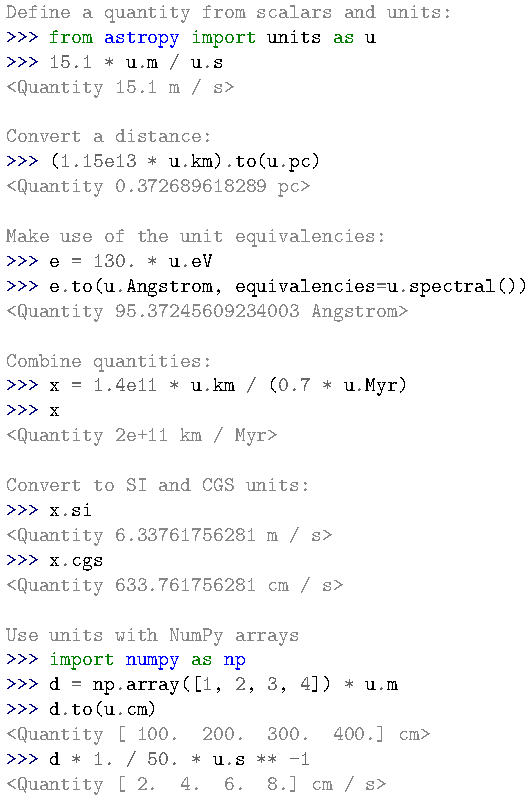
\includegraphics[scale=0.82,clip]{examples/code_quantities.pdf}}
\end{figure}

\subsubsection{Quantities and Physical Constants}

\label{sec:quantities}

While the previous section described the use of the units package to
manipulate the units themselves, a more common use-case is to attach
the units to quantities, and combine these. The \texttt{astropy.units}
package allows units to be attached to Python scalars, or \gls{numpy}
arrays, producing \texttt{Quantity} objects. These objects support
arithmetic with other numbers and \texttt{Quantity} objects and
preserve their units. For multiplication and division, the resulting
object will retain all units used in the expression.  The final object
can then be converted to a specified set of units or decomposed,
effectively canceling and combining any equivalent units and returning
a \texttt{Quantity} object in some set of base units. This is
demonstrated in Figure~\ref{code:quantities}:19.

Using the \texttt{.to()} method, \texttt{Quantity} objects can easily be
converted to different units. The units must either be dimensionally
equivalent, or users should pass equivalencies through the
\texttt{equivalencies} argument (c.f. \S\ref{sec:units}).

\begin{figure}
\caption{Using the \texttt{astropy.constants} sub-package.\label{code:constants}}
\fbox{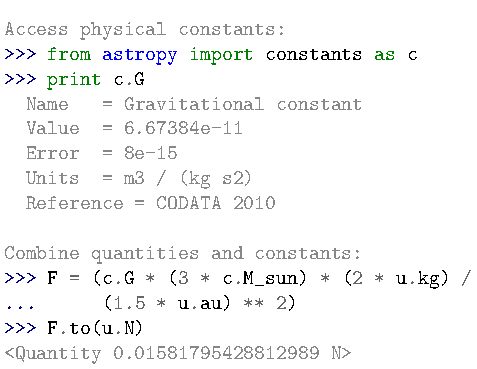
\includegraphics[scale=0.82,clip]{examples/code_constants.pdf}}
\end{figure}

\texttt{Quantity} objects (c.f. \S\ref{sec:quantities}) are used to
define a number of useful astronomical constants included with
Astropy, each with an associated unit (where applicable) and
additional metadata describing their provenance and
uncertainties. These can be used along with \texttt{Quantity} objects
to provide a convenient framework for computing any quantity in
Astronomy. Figure~\ref{code:constants} includes a simple example that
shows how the graviational force between two bodies can be calculated
in Newtons using physical quantities and user-specified quantities.

\subsection{Time}

% Authors: Tom A.

\begin{figure}
\caption{Time representation and conversion using the \texttt{astropy.time} sub-package.\label{code:time}}
\fbox{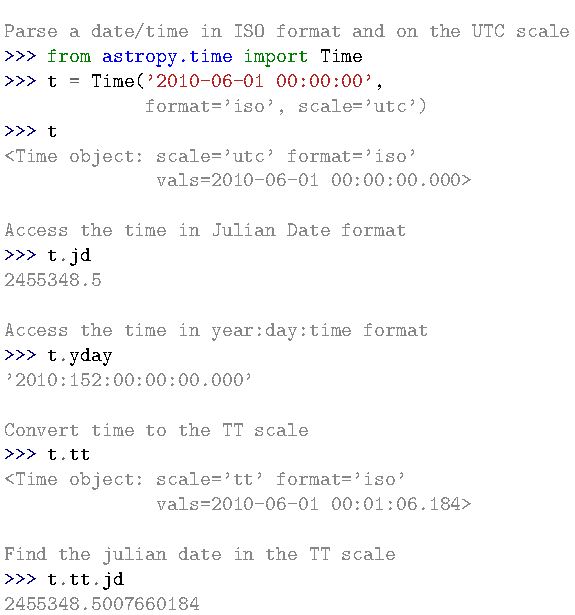
\includegraphics[scale=0.82,clip]{examples/code_time.pdf}}
\end{figure}

The \texttt{astropy.time} package provides functionality for manipulating
times and dates.  Specific emphasis is placed on supporting time scales
(e.g. UTC, TAI, UT1) and time formats/representations (e.g. JD, MJD, ISO 8601) that
are used in astronomy.

This package makes use of the Standards of Fundamental Astronomy (SOFA) time
and calendar library\footnote{\url{http://www.iausofa.org/}}. Leveraging the
robust and well-tested SOFA routines ensures that the fundamental time scale
conversions are being computed correctly. An important feature of the SOFA
time library is that each time is represented as a pair of double-precision
values. This is supported in \texttt{astropy.time} and provides the capability
to do extremely high precision time computations. All time scale conversions
are done by vectorized versions of the SOFA routines\footnote{using Cython
(\url{http://www.cython.org/})} and are reasonable fast and memory efficient.

The most common way to use \texttt{astropy.time} is to create a \texttt{Time} object
by supplying one or more input time values as well as the time format/representation
and time scale of those values. The input time(s) can either be a
single scalar like \verb|"2010-01-01 00:00:00"| or \verb|2455348.5| or a
sequence of such values; the format/representation specifies how to interpret the input
values, e.g. ISO or JD or Unix time; and the scale specifies the time standard
used for the values, e.g. UTC or TT or UT1. The available time scales are
listed in Table~\ref{tab:time_systems}.

\begin{table}
\caption{Supported time systems for \texttt{astropy.time}\label{tab:time_systems}}
\center
\begin{tabular}{ll}
\hline
Scale  & Description \\
\hline
TAI    & International Atomic Time \\
TCB    & Barycentric Coordinate Time \\
TCG    & Geocentric Coordinate Time \\
TDB    & Barycentric Dynamical Time \\
TT     & Terrestrial Time \\
UT1    & Universal Time \\
UTC    & Coordinated Universal Time \\
\hline
\end{tabular}
\end{table}

Getting the representation of a \texttt{Time} object in a different format
such as Julian Date is straightforward, as is converting to a different time
scale, for instance from UTC to TT (see Figure \ref{code:time}).

%Note that both the ISO and JD representations of \verb|t_tt| are different
%than for \verb|t| because they are expressed relative to the TT time scale.

Finally, in addition to representing absolute times, the \verb|Time| class supports
basic arithmetic to compute the duration between two times or to add or
subtract a duration from a time.

% Example that shows The example below also shows that when creating a
% \verb|Time| object the time format for unambiguous inputs can be
% automatically determined.

\subsection{Celestial Coordinates}

% Authors: Erik T., Adrian, Demitri

An essential element of any astronomy workflow is the manipulation, parsing,
and conversion of astronomical coordinates. This functionality is provided
in Astropy by
the \texttt{astropy.coordinates} sub-package. The aim of this package is to
provide a common application programming interface (API) for Python astronomy
packages that use coordinates, and to relieve users from having to
(re)implement extremely common utilities. To achieve this, it leverages
important lessons learned from existing Python coordinates packages such as
\texttt{kapteyn}, \texttt{pyast}, \texttt{pyephem} \citep{pyephem}, and
\texttt{astropysics} \citep{astropysics} that this package aims to supplant.

The package has been designed to present a natural Python interface for
representing coordinates in computations, simplify input/output formatting,
and allow straightforward transformation between coordinate systems. It also
supports implementation of new or custom coordinate systems that work
consistently with the built-in systems. A future design goal is to also
seamlessly support arbitrarily large data sets.

To that end, Figure \ref{fig:code_coordinates} shows some typical usage
examples for \texttt{astropy.coordinates}. Coordinate objects are 
created using standard Python object instantiation via
a Python class named after the coordinate system (e.g.,
\texttt{ICRSCoordinates}). Astronomical coordinates may be expressed in a
myriad of ways: the classes support string, numeric, and tuple value
specification through a sophisticated input parser. A design goal of the input 
parser is to be able to determine the angle value and unit from the input 
alone if a person can unambiguously determine them. For example, an
astronomer seeing the input string ``12h53m11.5123s'' would understand 
the units to be in hours, minutes, and seconds, so this value is alone 
sufficient to pass to the angle initializer. This functionality is build around
the \texttt{Angle} object, which can be instantiated and used on
its own. It provides additional functionality like string formatting and
mechanisms to specify the valid bounds of an angle.


\begin{figure}
\caption{Celestial coordinate representation and conversion.\label{code:coords}}
\fbox{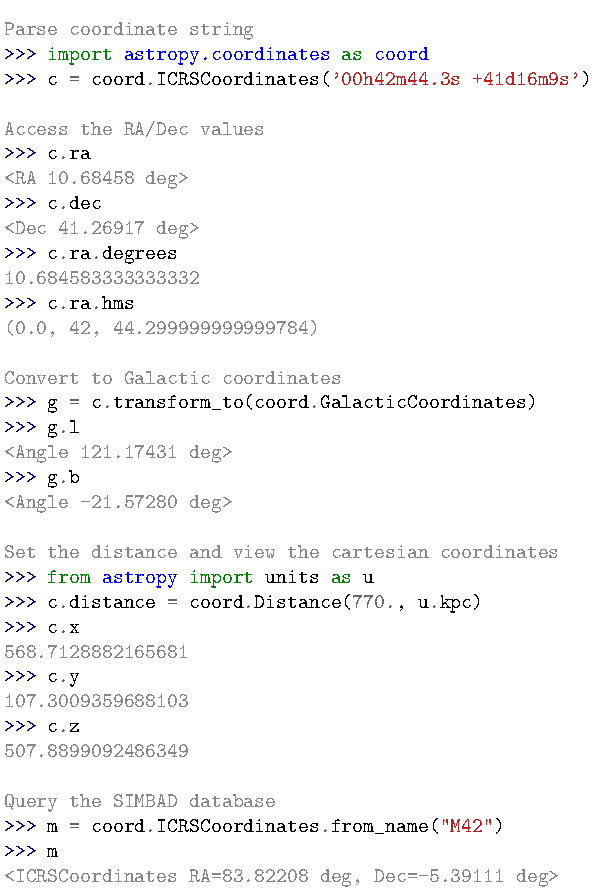
\includegraphics[scale=0.82,clip]{examples/code_coordinates.pdf}}
\label{fig:code_coordinates}
\end{figure}

The different coordinate classes represent different coordinate 
systems, and provide most of the user-facing
functionality for \texttt{astropy.coordinates}. The systems provide
customized initializers and appropriate formatting and representation
defaults. For some classes, they also contain added functionality specific to
a subset of systems, such as code to precess a coordinate to a new equinox.
The implemented systems include a variety of equatorial coordinate systems
(ICRS, FK4, and FK5), Galactic coordinates, and horizontal (Alt/Az)
coordinates. Future versions of Astropy will include additional common
systems, including ecliptic systems, supergalactic coordinates, and all
necessary intermediate coordinate systems for the IAU 2000/2006
equatorial-to-horizontal mapping \citep[e.g.,][]{soffel03, usnocircular179}.


Another major feature of \texttt{astropy.coordinates} is the methodology
for transforming between coordinate systems. Figure \ref{fig:code_coordinates} 
illustrates the most basic use of this functionality to convert from ICRS to 
Galactic coordinates.
Transformations are provided between all coordinate systems built into 
version 0.2 of Astropy, with the exception of conversions from
celestial to horizontal coordinates. This is planned for the next major
release, using  the transformation architecture endorsed by the IAU 
2000/2006 resolutions \citep[see e.g.,][]{soffel03, usnocircular179}. 

A final significant feature of \texttt{astropy.coordinates} is support for
line-of-sight distances. While the term ``celestial coordinates'' can be taken
to refer to only on-sky angles, in \texttt{astropy.coordinates} a coordinate
object is conceptually treated as a point in three dimensional space. Users
have the option of specifying a line of sight distance to the object from the
origin of the coordinate system (typically the origin is the Earth or solar
system barycenter). These distances can be given in physical units or as
redshifts. The \texttt{astropy.coordinates} package will in the latter case
transparently make use of the cosmological calculations in
\texttt{astropy.cosmology} (c.f. \S\ref{sec:cosmology}) for conversion to 
physical distances.  Figure \ref{fig:code_coordinates}  illustrates an
application of this information in the form of computing three-dimensional
distances between two objects.


These features are made more useful by the design philosophy of 
\texttt{astropy.coordinates} that it should be easy for a user to add 
new systems with minimal bookkeeping. In fact, it is possible
for a new contributor or user to add a new coordinate system with only a class
definition and two transformation functions. Coordinate systems added in this
manner are ``first-class citizens'' of the package, meaning that they have all
the capabilities of the systems that are included in the package. An 
example of such a user-defined system is provided in the 
documentation\footnote{\url{http://docs.astropy.org/en/v0.2/coordinates/sgr-example.html#complete-code-for-example}},
illustrating the definition of a coordinate system useful for a specific
scientific task (Johnston \& Price-Whelan 2013, in prep).


This flexibility is achieved in \texttt{astropy.coordinates} through the use
of a transformation graph. All coordinate systems are represented as classes;
internally, the transformation infrastructure keeps track of a network of
coordinate systems and the transformations between them. When a coordinate
object is to be transformed from one system into another, the package
determines the shortest path on the transformation graph to the new system and
applies the necessary sequence of transformations. Thus, implementing a new
coordinate system only requires implementing one pair of transformations to
and from a system that is already connected to the transformation graph. Once
this pair is specified, \texttt{astropy.coordinates} can transform from that
coordinate system to any other in the graph. This greatly simplifies
implementation and mirrors the way most coordinate systems are defined. For
example, Galactic coordinates are defined relative to FK4 coordinates rather
than with respect to a set of other common coordinate systems
\citep{galcoords, reid04}.





%\begin{verbatim}
%>>> from astropy.coordinates import Angle
%>>> a = Angle(118.439234, unit=u.degree)
%>>> a.radians
%2.067154596840014
%>>> a.hms
%(7.0, 53, 45.41616000000232)
%\end{verbatim}


%\begin{verbatim}
%>>> a = Angle(86.75309, unit=u.degree)
%>>> a.format()
%'86d45m11.12400s'
%>>> a.format(unit=u.hour, sep=':')
%'5:47:00.74160'
%>>> a.format(unit=u.hour, precision=2)
%'5h47m00.74s'
%\end{verbatim}

%
%\begin{verbatim}
%>>> Angle(275.439234, u.degree, bounds=(-180,180))
%<Angle -84.56077 deg>
%>>> Angle(-86.75309, u.degree, bounds=(0,360))
%<Angle 273.24691 deg>
%\end{verbatim}

\subsection{Tables and Gridded data}

% Authors: Tom A., Tom R., Wolfgang K., Erik T.

\label{sec:table}

\textbf{[TODO: examples of table creation and simple I/O]}\\

Tables and n-dimensional data arrays are the most common forms of data
encountered in astronomy. The \gls{python}-community has various solution for
tables, such as \gls{numpy} structured arrays or \texttt{DataFrame} objects in Pandas\footnote{\url{http://pandas.pydata.org}} to name
only a couple. For the n-dimensional data array Python brings their own
\texttt{array} class, in addition to the very popular \gls{numpy}
\texttt{ndarray}.

However, for use in astronomy all of these implementations lack some key
features. The data that is stored in arrays and tables does most often contain
vital metadata: the data is associated with units, and might also contain
additional arrays that either mask or provide additional attributes to each
cell. Furthermore, the data often has a parameter/value dataset attached with
it. Finally, the data comes in a plethora of astronomy specific formats (fits,
specially formatted ascii tables, etc. ) which are not recognized by the
pre-existing packages.

The \texttt{astropy.table} and \texttt{astropy.nddata} sub-packages contain
classes (\texttt{Table} and \texttt{NDData}) that try to alleviate these problems.
They allow users to represent astronomical data in the form of tables or
n-dimensional gridded datasets, including all meta-data.

The \texttt{Table} class provides a high-level wrapper to Numpy structured
arrays, which are essentially arrays that have fields (or columns) with
heterogeneous data types, and any number of rows. Numpy structured arrays are
however difficult to manipulate or modify, so the \texttt{Table} class makes
it easy for users to create a table from columns, add/remove columns or rows,
and mask values from the table. Furthermore, tables can be easily read/written
from/to common file formats using the \texttt{Table.read} and
\texttt{Table.write} methods. In addition to providing easy manipulation and
input/output of table objects, the \texttt{Table} class allows units to be
specified for each column using the \texttt{astropy.units} framework, and also
allows the \texttt{Table} object to contain arbitrary meta-data (stored in
\texttt{Table.meta}).

The \texttt{NDData} class provides a way to easily store n-dimensional array
data and builds upon the \gls{numpy} \texttt{ndarray} class. The actual data
is stored in just a \texttt{ndarray}, which allows for easy compatibility with
other scientific packages. In addition to parameter/value meta-data, the
\texttt{NDData} class can store a boolean mask with the same dimensions as the
data, several sets of flags (n-dimensional arrays that store attributes for
each cell of the data array), uncertainties, units, and a transformation
between array-index coordinate system and other coordinate systems (c.f.
\S\ref{sec:wcs}). In addition, the \texttt{NDData} class intends to provide
methods to arithmetically combine the data in a meaningful way.
\texttt{NDData} is not meant for direct user interaction but more for
providing a framework for higher-level subclasses like a spectrum class or an
astronomical image class. The \texttt{NDData} class currently does not have any built-in readers
and writers.

\subsection{File Formats}


\subsubsection{FITS}

% Authors: Erik B.

\label{sec:fits}

Support for reading and writing FITS files is provided by the
\texttt{astropy.io.fits} sub-package which, at the time of writing, is a
direct port of the
PyFITS\footnote{\url{http://www.stsci.edu/institute/software_hardware/pyfits}}
project \citep{barrett1999pyfits}. Users already familiar with PyFITS will
therefore feel at home with this package. Figure~\ref{code:fits} shows an example of how to
open an existing FITS file, access and modify the header and data, and write a new file back to disk.

\begin{figure}
\caption{Accessing data in FITS format.\label{code:fits}}
\fbox{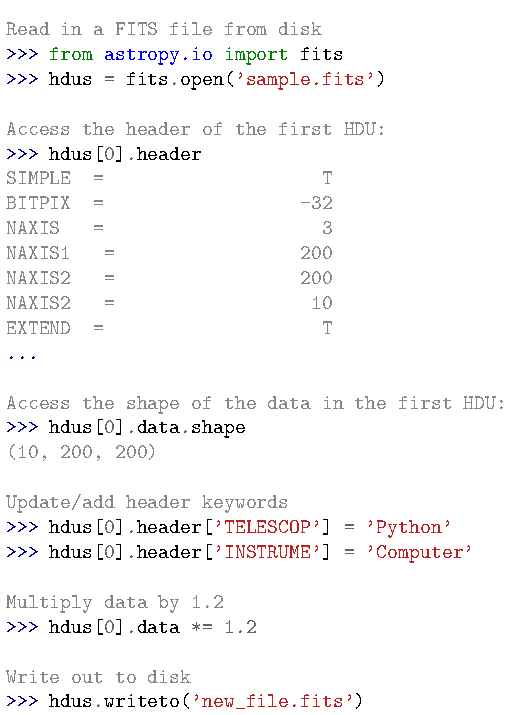
\includegraphics[scale=0.82,clip]{examples/code_fits.pdf}}
\end{figure}

Because the interface is exactly the same as that of PyFITS, users may directly
replace PyFITS with Astropy in existing code by changing import statements
like \texttt{import pyfits} to \texttt{from astropy.io import fits as pyfits}
without any additional code changes.

Although PyFITS will continue to be released as a separate product in the near
term, the long term plan is to discontinue PyFITS releases in favor of Astropy.
The exact timing of when PyFITS releases will be discontinued is not settled,
but users of PyFITS should plan to make suitable changes to support the eventual
transition to Astropy.

Becoming integrated with Astropy as the \texttt{astropy.io.fits} package will
greatly enhance future development on the existing PyFITS code base in several
areas.  First and perhaps foremost is integration with Astropy's \texttt{Table}
interface which is much more flexible and powerful than PyFITS' current
table interface.
We will also be able to integrate Astropy's unit support in order to attach
units to FITS table columns as well as header values that specify units in
their comments in accordance with the FITS standard.  Finally, as the PyWCS
package has also been integrated into Astropy as \texttt{astropy.wcs}
(c.f. \S\ref{sec:wcs}) tighter association between data from FITS files and their world coordinate system (WCS)
will be possible.


\subsubsection{ASCII table formats}
\label{sec:ascii}
% Authors: Tom A.

The \texttt{astropy.io.ascii} sub-package (formerly the standalone project
\texttt{asciitable}\footnote{\url{https://asciitable.readthedocs.org}}) provides the
ability to read and write tabular data for a wide variety of ASCII-based
formats.  In addition to generic formats such as space-delimited, tab-delimited or
comma-separated values, \texttt{astropy.io.ascii} provides classes for specialized
table formats like
CDS\footnote{\url{http://vizier.u-strasbg.fr/doc/catstd.htx}},
IPAC\footnote{\url{http://irsa.ipac.caltech.edu/applications/DDGEN/Doc/ipac_tbl.html}},
IRAF DAOphot, and LaTeX.  There is also a flexible class for handling
a wide variety of fixed-width table formats. Finally, this package is designed to be extensible, making it easy for users to define their own readers/writers for any other ASCII formats.

% TODO: since these examples can be done with the high-level table interface, shall we showcase that instead and include examples of VO and ASCII?

%As a simple example, suppose the file named \verb|sources.dat| has the following
%table information:
%
%\begin{verbatim}
%obsid redshift  X      Y     object
%3102  0.32      4167  4085   Q1250+568-A
%877   0.22      4378  3892   "Source 82"
%\end{verbatim}
%
%This table can be read with the following:
%
%\begin{verbatim}
%>>> from astropy.io import ascii
%>>> data = ascii.read("sources.dat")
%>>> print data
%obsid redshift  X    Y      object
%----- -------- ---- ---- -----------
% 3102     0.32 4167 4085 Q1250+568-A
%  877     0.22 4378 3892   Source 82
%\end{verbatim}
%
%This table can then be written out as a LaTeX table with the following:
%
%\begin{verbatim}
%>>> ascii.write(data, 'sources.tex',
%                Writer=ascii.Latex)
%>>> cat sources.tex
%\begin{table}
%\begin{tabular}{ccccc}
%obsid & redshift & X & Y & object \\
%3102 & 0.32 & 4167 & 4085 & Q1250+568-A \\
%877 & 0.22 & 4378 & 3892 & Source 82 \\
%\end{tabular}
%\end{table}
%\end{verbatim}
%
%As mentioned in Sec.~\ref{sec:table} there is an alternate way of
%reading and writing tables which is more intuitive in many cases.
%The previous example could be done with the following:
%
%\begin{verbatim}
%>>> from astropy.table import Table
%>>> data = Table.read('sources.dat',
%                      format='ascii')
%>>> data.write('sources.tex', format='ascii',
%               Writer=ascii.Latex)
%\end{verbatim}

\subsubsection{Virtual Observatory tables}

% Authors: Mike D.
The \texttt{astropy.io.votable} package (formerly the standalone project
\texttt{vo.table}) provides full support for reading and writing
VOTable format files versions 1.1 and 1.2
\citep{ochsenbein2004votable,ochsenbein2009votable}.  It efficently
stores the tables in memory as Numpy structured arrays.  The file is
read using streaming to avoid reading in the entire file at once and
greatly reducing the memory footprint.

It is possible to convert any one of the tables in a VOTable file to
a \texttt{Table} object (\S\ref{sec:table}), where it
can be edited and then written back to a VOTable file without any loss
of data.

The VOTable standard is not strictly adhered to by all VOTable file
writers in the wild.  Therefore, \texttt{astropy.io.votable} provides
a number of tricks and workarounds to support as many VOTable sources
as possible, whenever the result would not be ambiguous.  A validation
tool (\texttt{volint}) is also provided that outputs recommendations
to improve the standard compliance of a given file, as well as
validate it against the official VOTable schema.
Support for VOTable 1.3 is planned for the future.

\subsection{World Coordinate Systems}

\label{sec:wcs}

% Authors: Mike D.

The \texttt{astropy.wcs} package contains utilities for managing World Coordinate
System (WCS) transformations in FITS files.  These transformations map
the pixel locations in an image to their real-world units, such as
their position on the celestial sphere.  This library is specific to
WCS as it relates to FITS as described in the FITS WCS papers
\citep{greisen2002wcs,calabretta2002wcs,greisen2006wcs} and is
distinct from a planned Astropy package that will handle WCS
transformations in general, regardless of their representation.

This package is a wrapper around Mark Calabretta's
\texttt{wcslib} \citep{calabretta2013wcslib}.  Since all of the FITS
header parsing is done using \texttt{wcslib}, it is assured the same
behavior as the many other tools that use \texttt{wcslib}.  On top of
the basic FITS WCS support, it adds support for the Simple Imaging
Polynomial (SIP) convention and table lookup distortions as defined in
the draft WCS ``Paper IV'' \citep{calabretta2004wcs}.  Each of these
transformations can be used independently or together in a fixed
pipeline.

The \texttt{astropy.wcs} package also serves as a useful FITS WCS validation tool,
as it is able to report on many common mistakes or deviations from the
standard in a given FITS file.

\subsection{Cosmology}

\label{sec:cosmology}

% Authors: Neil Crighton, Alex Conley

The \texttt{astropy.cosmology} sub-package contains classes for
representing widely used cosmologies, and functions for calculating
quantities that depend on a cosmological model. It also contains a
framework for working with less frequently employed cosmologies that
may be not be flat, or have a time-varying pressure to density ratio,
$w$, for dark energy. The quantities that can be calculated are
generally taken from those described by \citet{Hogg99}. Some examples
are the angular diameter distance, comoving distance, critical
density, distance modulus, lookback time, luminosity distance, and
Hubble parameter as a function of redshift.

\begin{figure}
\caption{Cosmology utilities.\label{code:cosmology}}
\fbox{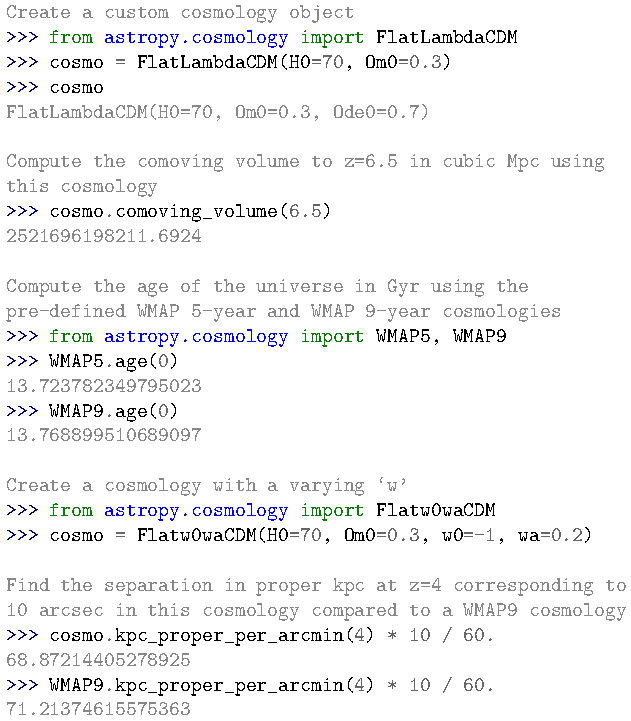
\includegraphics[scale=0.82,clip]{examples/code_cosmology.pdf}}
\end{figure}

The fundamental model for this sub-package is that any given cosmology
is represented by a class. An instance of this class has attributes
giving all the parameters required to uniquely specify the cosmology,
such as the Hubble parameter, CMB temperature and the baryonic, cold
dark matter, and dark energy densities at $z=0$. One can then use
methods of this class to perform calculations using these parameters.

Figure~\ref{code:cosmology} shows how \texttt{FlatLambdaCDM} can be
used to create an object representing a flat cosmology, and how the
methods of this object can be called to calculate the comoving volume,
age and transverse at a given redshift. Further calculations can be
performed using the many methods of the cosmology object as described
in the Astropy documentation. For users who are more comfortable using
a procedural coding style, these methods are also available as
functions that take a cosmology class instance as a keyword argument.

The sub-package provides several pre-defined cosmology instances
corresponding to commonly used cosmological parameter sets. Currently
parameters from the WMAP 5-year \citep{Komatsu09}, 7-year
\citep{Komatsu11} and 9-year results \citep{Hinshaw13} are included
(\texttt{WMAP5}, \texttt{WMAP7} and \texttt{WMAP9}).  There are
several classes corresponding to non-flat cosmologies, and the most
common dark energy models are supported: a cosmological constant,
constant $w$, and $w(a) = w_0 + w_a (1-a)$ (e.g. \citealt{Linder03},
here $a$ is the scale factor). Figure~\ref{code:cosmology} gives
examples showing how to use the pre-defined cosmologies, and how to
define a new cosmology with a time-varying dark energy $w(a)$. Any
other arbitrary cosmology can be represented by sub-classing one of
the basic cosmology classes.

All of the code in the sub-package is tested against the web-based
cosmology calculator by \citet{Wright06} and two other widely-used
calculators\footnote{\url{http://www.kempner.net/cosmic.php}}$^,$\footnote{\url{http://www.icosmos.co.uk/index.html}}.
In cases when these calculators are not precise enough to enable a
meaningful comparison, the code is tested against calculations
performed with \textsc{Mathematica}.

\section{Development workflow}

\label{sec:workflow}

% Describe tools used in the development process, and how development is managed (not specifically how we use git, but higher-level.

% Authors: Tom R., Erik T., Perry G.

In order to co-ordinate the development of Astropy by over 30 developers
worldwide, we have made use of the
GitHub\footnote{\url{http://www.github.com}} code collaboration platform. The
main repository for Astropy is stored in a
git\footnote{\url{http://git-scm.com/}} repository on GitHub, and any
non-trivial changes are made via \textit{pull requests}, which are a mechanism
for submitting code for review by other developers prior to merging into the
main code base. This workflow ensures that only high-quality, and well
documented and tested code is included into Astropy. Not all contributions are
necessarily accepted - community consensus is needed for incorporating major
new functionality in Astropy, and any new feature has to be justified to avoid
implementing features that are only useful to a minority of users, but may
cause issues in future.

At the time of writing, Astropy includes several thousand tests, which are
small units of code that check that functions/methods/classes in Astropy are
behaving as expected, both numerically, and from a usability point of view. We
make use of \textit{Continuous Integration}, which is the process of running
all the tests under various configurations (such as different versions of
Python or Numpy, and on different platforms) in order to ensure that the
package is held to the highest standard of stability. In particular, any
change made via a pull request is subject to extensive testing before being
merged into the core repository. For the latter, we make use of
Travis\footnote{\url{https://travis-ci.org/}}, while for running more
extensive tests across Linux, MacOS X, and Windows, we make use of
Jenkins\footnote{\url{http://jenkins-ci.org/}} (both are examples of Continuous Integration systems).

This development workflow has worked very well so far, allowing contributions
by many developers, and blurring the line between developers and users.
Indeed, users who encounter bugs and who know how to fix them can submit
suggested changes. We have also implemented a feature that means that anyone
reading the documentation at \url{http://docs.astropy.org} can suggest
improvements to the documentation without any prior knowledge of the
git version control system.

\section{Planned functionality}

\label{sec:future}

% Authors: Tom R., Erik T., Perry G.

Development on Astropy is very active, and we are focusing on several areas
for the next (0.3) release (some of which have already been implemented in the
publicly-available developer version):

\begin{itemize}
\item Seamlessly integrating the \texttt{Quantity} framework across all sub-packages
\item Supporting more file formats for reading and writing \texttt{Table} and \texttt{NDData} objects
\item Implementing a Virtual Observatory cone search tool
\item Implementing a generalized model-fitting framework
\end{itemize}

In the longer term, we are already planning the following functionality:

\begin{itemize}
\item More Virtual Observatory tools
\item A SAMP server/client (based on the SAMPy\footnote{\url{http://pythonhosted.org/sampy/}} package)
\item Aperture and PSF photometry tools
\item Spectroscopic analysis tools
\end{itemize}

\noindent and undoubtedly the core functionality will grow beyond this.

\section{Summary}

\label{sec:summary}

% Authors: Tom R., Erik T., Perry G.

We have presented the first public release of the Astropy package, a core
Python package for Astronomers. In this paper, we have described the main
functionality, which ranges from handling of common file formats in Astronomy,
data structures, unit conversions, and coordinate systems. We also briefly
described our development workflow and plans for the future. We encourage
members of the community to join the effort by adopting Astropy for their own
projects, reporting any issues, and whenever possible, developing new
functionality.

\bibliographystyle{apj_custom}
\bibliography{apj-jour,references}

\end{document}
